\chapter{Zusammenfassung}
\label{cap:summary}

\section{Einleitung}
\label{sec:introduction}

Kostenpflichtige Fernsehprogramme (folgend Pay-TV genannt) wie z.B. Sky (ehemals Premiere) oder wie in diesem Fall HD+\footnote{Hochauflösendes, kostenpflichtes Fernsehprogramm der privaten Sender RTL, ProSieben, etc.} werden über Satellit\footnote{Andere Übertragungsarten sind Kabel oder terrestrisch, also über Antenne.} verschlüsselt übertragen, so dass nur zahlende Abonnenten, die zur Entschlüsselung des Programms technisch befähigt wurden, das Fernsehprogramm anzeigen können.

Neben dem üblichen Empfangsgerät, wie z.B. einem Satelliten-Receivers, wird zur Entschlüsselung des Programms eine Smartcard benötigt. Eine Smartcard ist ein digitales Speichergerät in EC-Kartengröße, auf der digitale Schlüssel gespeichert sind und auf die mit speziellen Smartcard-Kartenlesegeräten zugegriffen werden kann. Im Fall des HD+ Fernsehempfangs erhält der Abonnent bei Abschluss des Mietvertrags eine Smartcard mit seinem persönlichen Schlüssel, mit dem er das kostenpflichtige Fernsehprogramm entschlüsseln kann. Die Smartcard wird dafür in einen kompatiblen Satelliten-Receiver mit integrierten Lesegerät eingelegt, welcher dann die Entschlüsselung vornimmt.

Pay-TV Anbieter gestatten den Empfang nur auf zertifizierten, also von Ihnen geprüften und freigegebenen Empfangsgeräten. Dadurch können sie technische Sperren wie z.B. das Verbot der Aufzeichnung von Fernsehprogrammen in den Geräten erzwingen.

Zudem ist die Anzahl der Empfangsgeräte, über welche Pay-TV angezeigt werden kann, über die Anzahl der ausgegebenen Smartcards limitiert. Ein Abonnent kann mit einer Smartcard also nur auf einem Fernsehgerät das Programm betrachten.

Der Tatverdächtige Max Mustermann soll gegen diese beiden Beschränkungen verstoßen haben: die Aufzeichnung von Pay-TV Inhalten und die Anzeige des Fernsehprogramms mit einer Smartcard auf mehreren Geräten, auch als \textit{Cardsharing} bekannt.

\section{Überblick über die analysierten PC-Systeme}
\label{sec:summary-overview}

Insgesamt wurden drei beschlagnahmte PC-Systeme des Tatverdächtigen Max Mustermann analysiert. Die \autoref{fig:summary-overview} gibt einen Überblick über diese Systeme, weitere angeschlossene Komponenten und die Verbindung der Systeme untereinander.

\begin{figure}[H]
\centering
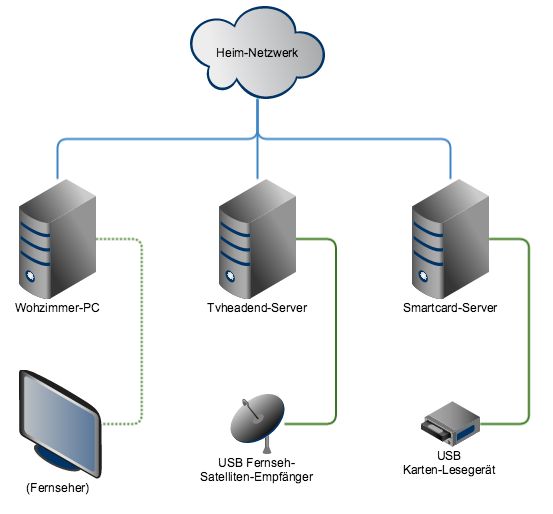
\includegraphics[scale=0.45]{system-overview.png} 
\caption{Überblick der analysierten Systeme und Beziehungen zueinander}
\label{fig:summary-overview}
\end{figure}

Alle drei Systeme sind über ein privates Computer-Heimnetzwerk (siehe blaue Verbindungen) miteinander verbunden, so dass sie Daten untereinander austauschen können. Zusätzlich sind weitere Komponenten an die Systeme angebunden (siehe grüne Verbindungen).

In den folgenden Abschnitten wird der Zweck der dargestellten Systeme und  Komponenten im Einzelnen erläutert.

\subsection{Wohnzimmer-PC}

Auf dem Wohnzimmer-PC wurde eine sogenannte Media-Center-Software namens \mbox{Kodi} betrieben. Eine Media-Center-Software ist eine PC-Software, mit der verschiedene Medien wie Fernseh- oder Radio-Übertragungen, Videos, Bilder, usw. über eine einfach zu nutzende Bedienoberfläche am PC abgespielt werden können. Bei Fernseh- und Radio-Übertragungen besteht zusätzlich die Möglichkeit diese aufzuzeichnen und später abzuspielen. In der Regel wird ein PC mit einer Media-Center-Software an einen Fernseher angeschlossen, so dass die Wiedergabe der Medien im großen Bildformat erfolgen kann. Da der Fernseher meist im Wohnzimmer steht, wird auch der PC dort aufgestellt und entsprechend genannt: Wohnzimmer-PC.

Da der Anschluss des Wohnzimmer-PCs an den Fernseher optional ist, wurde in der \autoref{fig:summary-overview} die grüne Verbindung entsprechend gepunktet dargestellt.

\subsection{Tvheadend-Server}

Um über einen PC Fernsehempfang zu ermöglichen, muss ein entsprechendes PC-kompatibles Fernseh-Empfangsgerät angeschlossen sein. In diesem Fall wurde der Empfang über ein externes USB\footnote{USB ist ein Standard für den Anschluss von externen Geräten an einem PC, siehe USB-Stick.}-Gerät für den Empfang von Satellitenfernsehen eingesetzt. Dieses Empfangsgerät war am zweiten PC-System angeschlossen, welches in \autoref{fig:summary-overview} als Tvheadend-Server bezeichnet ist. Neben dem Empfangsgerät (Hardware) ist auch eine Software für den Fernsehempfang erforderlich. In diesem Fall kam die Software Tvheadend zum Einsatz, nachdem auch das PC-System benannt wurde.

Um das Fernsehbild auch über die Media-Center-Software auf dem Wohnzimmer-PC anzuzeigen und zu steuern (z.B. umschalten, aufzeichnen), muss das am Tvheadend-Server empfangene Fernsehbild zum Wohnzimmer-PC übertragen werden. Dies erfolgte über das eingangs erwähnte private Heimnetzwerk, welches alle drei Systeme miteinander verband.

\subsection{Smartcard-Server}

Wie in \autoref{sec:introduction} erläutert, wird für die Entschlüsselung von Pay-TV Inhalten eine Smartcard vom Pay-TV Anbieter benötigt. Dies gilt auch für die Darstellung von Pay-TV Inhalten auf einem PC. 

Am dritten, der in \autoref{fig:summary-overview} als Smartcard-Server bezeichnete PC-System wurde ein USB-Kartenlesegerät für Smartcards betrieben. Zusätzlich war eine spezielle Software auf dem PC installiert, die einen geteilten Zugriff auf die Smartcard über das private Heim-Netzwerk ermöglicht. Geteilter Zugriff bedeutet technisch, dass eine Vielzahl von Empfangssystemen auf nur eine Smartcard zugreifen können. Die vom Pay-TV Anbieter vorgegebene Kopplung zwischen einer Smartcard und einem Empfangsgeräts ist damit technisch ausgehebelt.

Die Software Tvheadend für den Empfang von Fernsehinhalten hat eine Unterstützung für einen solchen über ein Netzwerk zur Verfügung gestellten Smartcard-Server integriert. Das bedeutet, dass die Software in der hier dargestellten Konstellation in der Lage ist Pay-TV Inhalte auf dem PC zu entschlüsseln und auf dem Wohnzimmer-PC zu übertragen. Die Media-Center-Software auf dem Wohnzimmer-PC kann diese Inhalte dann ausgeben oder auch aufnehmen.

\section{Sichergestellte Spuren}

Zur Belegung für die in \autoref{sec:summary-overview} dargestellten Umgehung der technischen Sicherheitsmechanismen des PayTV-Anbieters (Cardsharing) wurden die aufgefunden Spuren auf den untersuchten Systemen in \autoref{table:summary-traces} zusammengefasst.

\begin{table}
\begin{tabular}{p{0.3cm}p{3cm}p{9cm}p{1.1cm}}
\toprule
Nr. & System & Spur & Kapitel \\ 
\toprule
1. & Wohnzimmer-PC & Installiertes Softwarepakete des Media-Centers Kodi & 3.1.5 \\ 
\hline
2. & Wohnzimmer-PC & Installiertes Softwarepaket der Kodi Erweiterung zur Anbindung an Tvheadend & 3.1.5 \\ 
\hline
3. & Wohnzimmer-PC & Protokollierte Nutzung von Kodi am 04.05.2015 von 21:44 bis 21:59 Uhr & 3.1.6 \\ 
\hline
4. & Wohnzimmer-PC & Protokollierte Auswahl von HD+ Fernsehsender über Kodi am 04.05.2015 von 21:51 bis 21:58 Uhr & 3.1.6 \\ 
\hline
5. & Wohnzimmer-PC & Konfigurationsdateien zur Anbindung von Kodi an Tvheadend & 3.1.7 \\ 
\hline
6. & Tvheadend-Server & Installierte Softwarepakete von Tvheadend & 3.2.5 \\ 
\hline
7. & Tvheadend-Server & Videodatei mit kurzer Aufnahme der \textit{Wer wird Millionär?}-Spezialfolge auf dem RTL HD+ Sender am 04.05.2015 um 21:57 Uhr, siehe \autoref{fig:tvheadend-rtlhd} & 3.2.6 \\ 
\hline
8. & Tvheadend-Server & Übereinstimmung der Erstellungszeit der Aufnahme in Spur 7 mit dem protokollierten Nutzungszeitfenster von Kodi in Spur 3 & 3.2.6 \\ 
\hline
9. & Tvheadend-Server & Übereinstimmung der zeitlichen Abfolge der Kanalwechsel und Verweildauer auf den HD+ Sendern aus Spur 4 und der protokollierten Wiedergabe der Sender auf dem Tvheadend-Server & 3.2.7 \\ 
\hline
10. & Tvheadend-Server & Protokollierte Kommunikation zwischen der Tvheadend Software und dem Smartcard-Server & 3.2.8 \\ 
\hline
11. & Tvheadend-Server & Konfigurationsdateien zur Anbindung von Tvheadend an den Smartcard-Server & 3.2.8 \\ 
\hline
12. & Smartcard-Server & Quelldateien zur Installation der Smartcard Software & 3.3.4 \\ 
\hline
13. & Smartcard-Server & Installierte Programmdateien der Smartcard Software & 3.3.4 \\
\hline
14. & Smartcard-Server & Protokollierte Nutzung der Smartcard Software am 04.05.2015 von 19:45 bis 20:01 Uhr & 3.3.5 \\
\hline
15. & Smartcard-Server & Protokollierte Nutzung eines Kartenlesegeräts mit eingelegter HD+ Smartcard am 04.05.2015 um 19:45 Uhr & 3.3.5 \\
\hline
16. & Smartcard-Server & Protokollierte Verbindung von Tvheadend mit dem Smartcard Server am 04.05.2015 um 19:55 Uhr & 3.3.5 \\
\hline
17. & Smartcard-Server & Protokollierte Lesezugriffe auf die HD+ Smartcard im Zeitfenster der Aufnahme in Spur 7 am 04.05.2015 um 19:55 bis 19:58 Uhr & 3.3.5 \\
 \bottomrule
\end{tabular}
\caption{Liste der aufgefundenen Spuren auf den untersuchten Systemen}
\label{table:summary-traces}
\end{table}